% ============================================================
%  CHAPITRE 1 — ÉTUDE PRÉLIMINAIRE
% ============================================================
\chapter{Étude préliminaire}

\vspace{-0.5cm}
\begin{tcolorbox}[colback=lightgray, colframe=primaryblue, title=\textbf{Plan du chapitre}, fonttitle=\bfseries]
  \begin{enumerate}[leftmargin=*, label=\arabic*.]
    \item Présentation de l'organisme d'accueil \dotfill \pageref{sec:organisme}
    \item Contexte et Cadre du projet \dotfill \pageref{sec:cadre}
    \item Étude et critique de l'existant \dotfill \pageref{sec:existant}
    \item Les fondements intelligents de SmartPM \dotfill \pageref{sec:piliers}
    \item Étude de faisabilité et gestion des risques \dotfill \pageref{sec:faisabilite}
    \item Méthodologie et planification du projet \dotfill \pageref{sec:methodologie}
  \end{enumerate}
\end{tcolorbox}

% ─────────────────────────────────────────────────────────
\section*{Introduction}
% ─────────────────────────────────────────────────────────

Dans ce chapitre, nous présentons le contexte général dans lequel le projet a été conçu et
réalisé. Nous commençons par la présentation de l'organisme d'accueil, Capgemini Tunisie, 
puis nous explorons l'évolution de la gestion de projet moderne et l'apport crucial de 
l'Intelligence Artificielle (IA). Nous définissons ensuite les objectifs poursuivis, les enjeux 
associés et le périmètre du travail. Nous procédons par la suite à une analyse critique des 
solutions existantes afin d'en identifier les insuffisances, notamment en matière d'automatisation intelligente,
pour mettre en évidence la valeur ajoutée de SmartPM. Enfin, nous abordons l'étude de faisabilité,
les risques potentiels, ainsi que la méthodologie de travail agile adoptée pour mener à bien ce projet.

% ─────────────────────────────────────────────────────────
\section{Présentation de l'organisme d'accueil}
\label{sec:organisme}
% ─────────────────────────────────────────────────────────

\textbf{Capgemini} est l'un des leaders mondiaux du conseil, des services technologiques et
de la transformation digitale. Présent dans plus de 50 pays et fort de plus de 350~000
collaborateurs, le groupe accompagne ses clients dans la définition et la mise en œuvre de
leurs stratégies numériques, en exploitant la puissance des technologies cloud, de l'intelligence
artificielle, de la cybersécurité et de l'ingénierie logicielle.

\vspace{0.3cm}

\textbf{Capgemini Tunisie} est un centre de services offshore stratégique du groupe, implanté
à Tunis. Il regroupe des ingénieurs spécialisés dans le développement logiciel, l'architecture
des systèmes d'information, le DevOps et l'intelligence artificielle. La filiale tunisienne
intervient sur des projets de grande envergure pour des clients internationaux, notamment
dans les secteurs de l'aéronautique, de la finance, des télécommunications et de l'industrie.

\vspace{0.3cm}

Les domaines d'expertise de Capgemini Tunisie incluent :

\begin{itemize}
  \item Développement et intégration de solutions logicielles sur mesure
  \item Transformation digitale et conseil en stratégie IT
  \item Infrastructures Cloud et solutions DevOps (Docker, Kubernetes, CI/CD)
  \item Intelligence artificielle et data engineering
  \item Cybersécurité et gestion des identités (IAM)
\end{itemize}

\begin{figure}[H]
  \centering
  \includegraphics[width=6cm]{"images/logo_capgemini (2).png"}
  \caption{Logo de Capgemini}
  \label{fig:logo_capgemini}
\end{figure}

\subsection{Organisation de l'\'equipe projet}

L'équipe projet au sein de Capgemini Tunisie adopte une structure rigoureuse inspirée à la fois des méthodes agiles et des cycles de développement stricts requis par les projets de grande envergure (comme ceux encadrés par la norme DO-178C dans l'aéronautique). Comme l'illustre la Figure \ref{fig:organigramme}, la répartition des tâches garantit une séparation claire entre la spécification, le développement et la vérification.

\begin{figure}[H]
  \centering
  \begin{tikzpicture}[
      scale=0.95, transform shape, % Taille ajustée pour être parfaite (ni trop grand ni trop petit)
      leader/.style={
          draw=primaryblue, thick, rounded corners=6pt, 
          fill=primaryblue, text=white, 
          minimum width=5.5cm, minimum height=1.5cm, 
          align=center, font=\normalsize
      },
      pole/.style={
          draw=primaryblue!50, thick, rounded corners=6pt, 
          fill=white, text=darkgray,
          minimum width=5cm, minimum height=2.5cm, 
          align=center, font=\small
      },
      line/.style={
          draw=primaryblue!80, very thick, -stealth, rounded corners=4pt
      }
  ]
      % Direction
      \node[leader] (cp) at (0, 0) {\textbf{Direction de Projet} \\[0.1cm] \small Pilotage, Suivi Agile \& Qualit\'e};
      
      % Pôles
      \node[pole] (spec) at (-5.8, -3.5) {
          \textbf{\color{primaryblue} P\^ole Sp\'ecifications}\\[0.1cm]
          \textit{\color{gray} (Analyse des besoins)}\\[0.3cm]
          D\'efinition des exigences\\
          \& Architecture syst\`eme
      };
      
      \node[pole] (dev) at (0, -3.5) {
          \textbf{\color{primaryblue} P\^ole D\'eveloppement}\\[0.1cm]
          \textit{\color{gray} (Ingénierie logicielle)}\\[0.3cm]
          Codage, IA, DevOps\\
          \& Tests unitaires
      };
      
      \node[pole] (test) at (5.8, -3.5) {
          \textbf{\color{primaryblue} P\^ole V\'erification (V\&V)}\\
          \textit{\color{gray} (Assurance Qualité)}\\[0.3cm]
          Ex\'ecution des tests\\
          \& Validation finale
      };
      
      % Lignes de liaison
      \draw[line] (cp.south) -- (0, -1.8) -| (spec.north);
      \draw[line] (cp.south) -- (dev.north);
      \draw[line] (cp.south) -- (0, -1.8) -| (test.north);
  \end{tikzpicture}
  \caption{Organigramme de l'\'equipe projet}
  \label{fig:organigramme}
\end{figure}


% ─────────────────────────────────────────────────────────
\section{Contexte et Cadre du projet}
\label{sec:cadre}
% ─────────────────────────────────────────────────────────

\subsection{Évolution de la gestion de projet et l'apport de l'IA}

La gestion de projet logiciel a considérablement évolué ces dernières décennies, passant de 
modèles séquentiels traditionnels (Cycle en V, Cascade) vers des approches Agiles (Scrum, Kanban) 
privilégiant la flexibilité et la réactivité. Cependant, avec l'augmentation du volume de données 
et la complexité croissante des architectures logicielles modernes, les équipes de développement font face à de nouveaux défis :
surcharge informationnelle, suivi fastidieux de multiples tâches, et temps excessif consacré à la rédaction 
de rapports et aux réunions de synchronisation.

Dans ce contexte de digitalisation accélérée, l'Intelligence Artificielle Générative (IA) 
représente un changement de paradigme majeur. Elle ne se limite plus à de simples suggestions, 
mais agit comme un véritable assistant capable de synthétiser des informations complexes, de 
prédire des retards, de générer des bilans d'avancement et d'interagir naturellement avec les 
chefs de projet. C'est la transition de la gestion de projet "passive" vers la gestion de projet "intelligente".

\subsection{Objectif du projet}

L'enjeu principal du projet \textbf{SmartPM} est de fournir aux entreprises et aux équipes de 
développement une plateforme de gestion de projet de nouvelle génération. Ses objectifs principaux sont :

\begin{itemize}
  \item \textbf{Centraliser la gestion agile :} Gérer les projets, sprints, activités et tâches au sein d'une interface unifiée et intuitive.
  \item \textbf{Intégrer nativement l'IA (Generative AI) :} Doter la plateforme d'un assistant conversationnel contextuel capable de comprendre l'état du projet et de répondre aux requêtes en temps réel.
  \item \textbf{Automatiser la documentation :} Générer automatiquement des bilans de sprints et des synthèses de tâches grâce aux Large Language Models (LLM).
  \item \textbf{Garantir une robustesse Cloud-Native :} Déployer l'ensemble de la solution sur une infrastructure Kubernetes avec une observabilité complète (Prometheus, Grafana).
\end{itemize}

\subsection{Problématique}

La fragmentation des outils actuels oblige souvent les équipes à jongler entre des gestionnaires 
de tâches, des plateformes de communication et des outils d'analyse de données distincts. 
De plus, la majorité des outils du marché intègrent l'IA de manière superficielle (simples plugins), 
sans réelle compréhension du cycle de vie global du projet.

Cette situation soulève la problématique centrale suivante :

\begin{notebox}
  \textbf{Comment concevoir et déployer une plateforme web unifiée et Cloud-Native, intégrant au cœur 
  de son architecture une Intelligence Artificielle générative capable d'assister les équipes 
  dans la gestion de leurs projets agiles, tout en garantissant performance et scalabilité via DevOps ?}
\end{notebox}


% ─────────────────────────────────────────────────────────
\section{Étude et critique de l'existant}
\label{sec:existant}
% ─────────────────────────────────────────────────────────

\subsection{Analyse des solutions actuelles}

Avant de concevoir SmartPM, nous avons réalisé une étude comparative des principales
solutions de gestion de projets disponibles sur le marché, en évaluant particulièrement 
leur niveau d'automatisation, leur intégration de l'intelligence artificielle et leur flexibilité.

\vspace{0.3cm}

\textbf{Jira (Atlassian) :} Outil incontournable dans l'industrie, Jira excelle dans la gestion des sprints Scrum, le suivi des bugs et les tableaux Kanban. 
\textit{Limites :} Bien qu'il propose de multiples intégrations, Jira reste lourd à configurer. L'intelligence artificielle (Atlassian Intelligence) y est récente et fonctionne davantage comme un module complémentaire plutôt que comme un assistant conversationnel proactif capable d'interroger la totalité du cycle de vie du projet en langage naturel.

\vspace{0.3cm}

\textbf{Monday.com :} Plateforme collaborative moderne reconnue pour son interface très intuitive et visuelle. Elle permet une excellente gestion des tâches et une personnalisation poussée des flux de travail.
\textit{Limites :} Monday.com cible un usage très généraliste (marketing, RH, etc.). Elle manque de fonctionnalités natives dédiées exclusivement à l'ingénierie logicielle complexe et son moteur d'IA reste limité à la génération de textes ou la création de sous-tâches simples.

\vspace{0.3cm}

\textbf{Asana et Trello :} Ce sont des outils agiles très populaires pour leur simplicité d'utilisation (notamment la vue Kanban pour Trello).
\textit{Limites :} Ils ne sont pas conçus pour des projets logiciels de très grande envergure. Ils manquent de fonctionnalités DevOps natives, ne possèdent pas de métriques de suivi logiciel approfondies, et n'intègrent pas de LLMs pour l'analyse prédictive des projets.

\vspace{0.3cm}

\textbf{Microsoft Project :} Outil robuste et classique de planification, très utilisé pour la création de diagrammes de Gantt détaillés et le suivi des coûts.
\textit{Limites :} Il reste perçu comme un outil lourd, peu adapté à l'agilité moderne (Scrum). Il n'offre pas d'assistant IA natif et sa prise en main par les équipes de développement technique est souvent laborieuse.

\subsection{Critique de l'existant et justification de SmartPM}

L'analyse des solutions existantes démontre que si les outils actuels répondent parfaitement 
au besoin de suivi "manuel" des tâches, ils présentent un retard significatif en matière d'automatisation intelligente 
et d'infrastructures Cloud-Native intégrées.

\begin{table}[H]
  \centering
  \caption{Tableau comparatif des solutions existantes orientées IA \& DevOps}
  \label{tab:comparatif}
  \renewcommand{\arraystretch}{1.4}
  \begin{tabularx}{\textwidth}{|l|X|X|X|X|}
    \hline
    \rowcolor{tablehead}
    \textcolor{white}{\textbf{Critère}} &
    \textcolor{white}{\textbf{Jira}} &
    \textcolor{white}{\textbf{Monday}} &
    \textcolor{white}{\textbf{Asana}} &
    \textcolor{white}{\textbf{SmartPM}} \\
    \hline
    Gestion Agile (Scrum/Kanban) & \textcolor{successgreen}{\ding{51}} & \textcolor{successgreen}{\ding{51}} & \textcolor{successgreen}{\ding{51}} & \textcolor{successgreen}{\ding{51}} \\
    \hline
    Assistant IA conversationnel (RAG) & \textcolor{red}{\ding{55}} (Basique) & \textcolor{red}{\ding{55}} & \textcolor{red}{\ding{55}} & \textcolor{successgreen}{\ding{51}} \\
    \hline
    Génération automatique de bilans & \textcolor{red}{\ding{55}} & \textcolor{red}{\ding{55}} & \textcolor{red}{\ding{55}} & \textcolor{successgreen}{\ding{51}} \\
    \hline
    Architecture DevOps / Cloud-Native & \textcolor{red}{\ding{55}} (SaaS fermé) & \textcolor{red}{\ding{55}} (SaaS) & \textcolor{red}{\ding{55}} (SaaS) & \textcolor{successgreen}{\ding{51}} (K8s) \\
    \hline
    Monitoring intégré (Prometheus/Grafana) & \textcolor{red}{\ding{55}} & \textcolor{red}{\ding{55}} & \textcolor{red}{\ding{55}} & \textcolor{successgreen}{\ding{51}} \\
    \hline
    Open Source / Auto-hébergeable & \textcolor{red}{\ding{55}} & \textcolor{red}{\ding{55}} & \textcolor{red}{\ding{55}} & \textcolor{successgreen}{\ding{51}} \\
    \hline
  \end{tabularx}
\end{table}


% ─────────────────────────────────────────────────────────
\section{Les fondements intelligents de SmartPM}
\label{sec:piliers}
% ─────────────────────────────────────────────────────────

Pour pallier les limites des solutions du marché, \textbf{SmartPM} se positionne non pas comme un simple 
gestionnaire de tâches, mais comme une plateforme de gestion intelligente reposant sur trois piliers fondamentaux :

\begin{itemize}
  \item \textbf{L'Assistant IA Multi-modèles (Le cœur intelligent) :} SmartPM intègre un chatbot contextuel 
  s'appuyant sur les technologies RAG (Retrieval-Augmented Generation). En connectant directement les bases 
  de données MongoDB aux APIs de grands modèles de langage (Groq, Gemini, OpenRouter), l'assistant est capable 
  de répondre à des questions complexes telles que : \textit{"Quel est l'avancement du Sprint 2 ?"} ou \textit{"Génère un résumé des tâches de la semaine"}.

  \item \textbf{Gestion multi-rôles avancée et centralisée :} Trois niveaux d'accès distincts (Admin, Manager, Member) 
  permettent de structurer l'entreprise. La plateforme permet une hiérarchisation claire : Projet $\rightarrow$ Activité $\rightarrow$ Sous-Activité $\rightarrow$ Tâche, facilitant ainsi la visibilité globale.

  \item \textbf{Infrastructure DevOps robuste et moderne :} Conscients des besoins de haute disponibilité des entreprises, 
  nous avons conçu SmartPM pour être entièrement "Cloud-Native". L'application est containerisée via Docker et orchestrée 
  par Kubernetes (K8s). Un système de monitoring complet (Prometheus et Grafana) assure la surveillance en temps réel de la santé de l'application.
\end{itemize}

\vspace{0.5cm}
\begin{figure}[H]
  \centering
  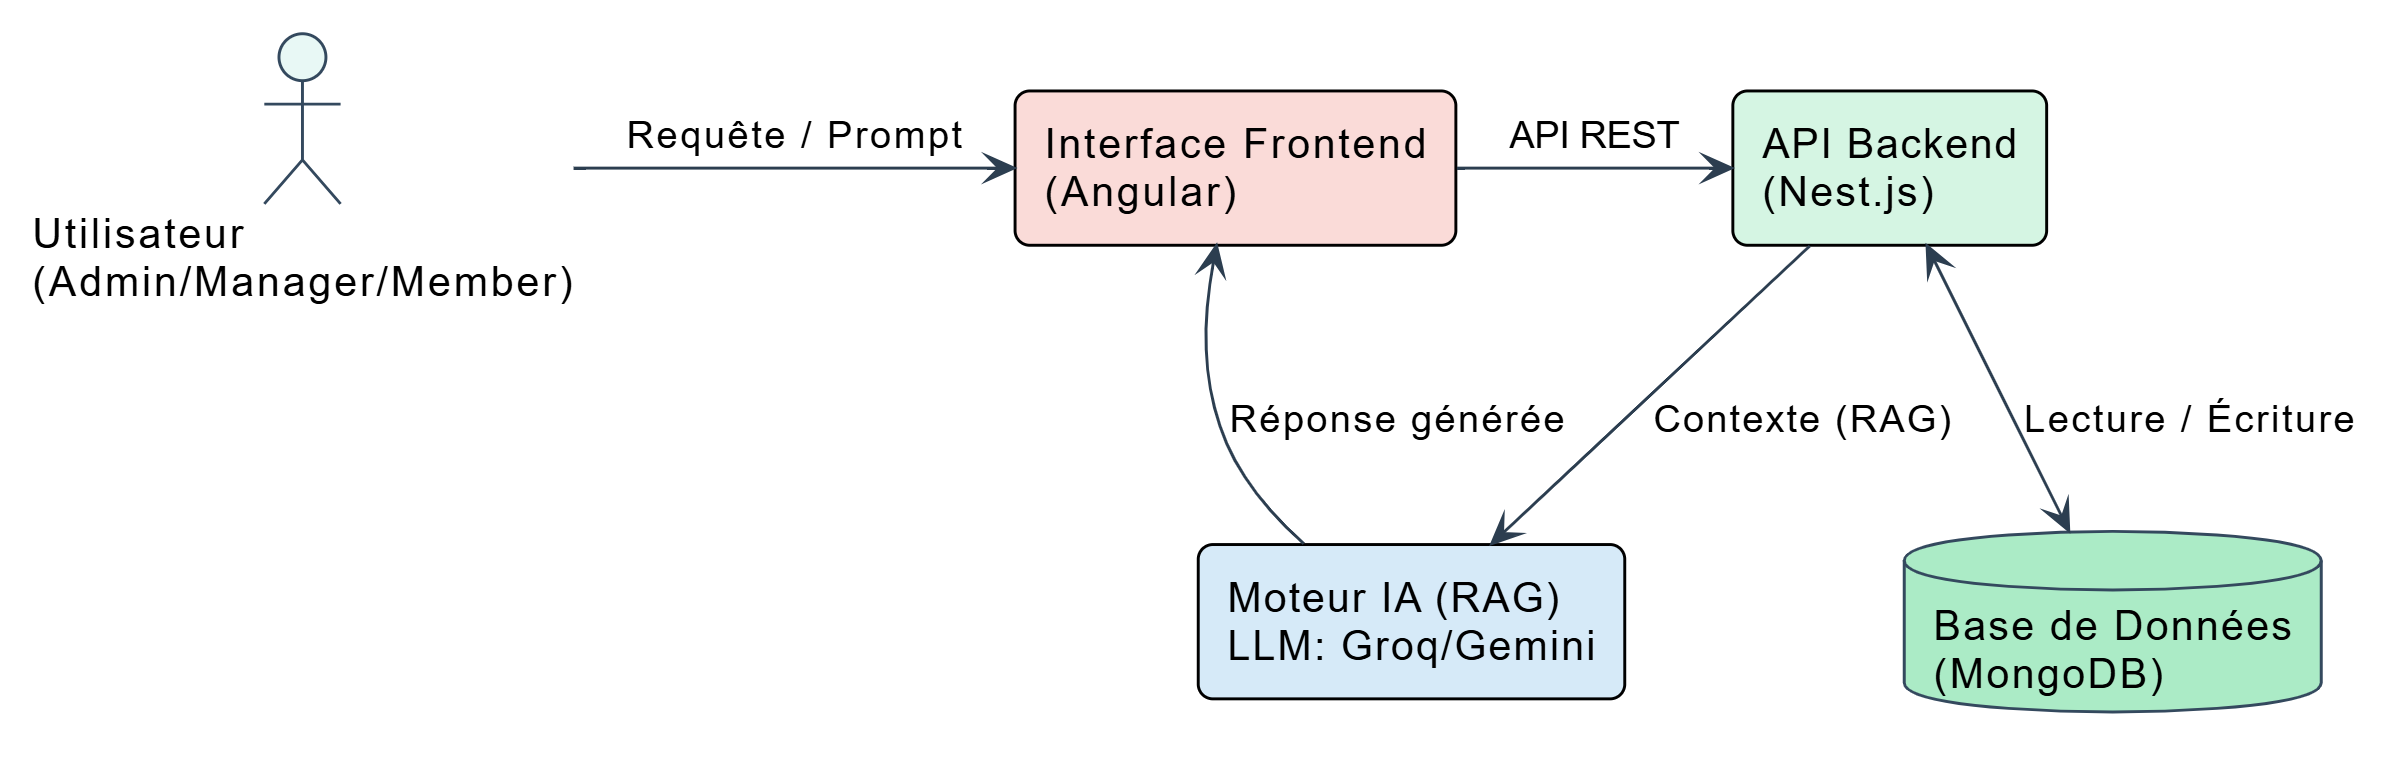
\includegraphics[width=0.9\textwidth]{images/flux_macroscopique.png}
  \caption{Diagramme de flux macroscopique de l'architecture intelligente SmartPM}
  \label{fig:flux_macroscopique}
\end{figure}
\vspace{0.3cm}


% ─────────────────────────────────────────────────────────
\section{Étude de faisabilité et gestion des risques}
\label{sec:faisabilite}
% ─────────────────────────────────────────────────────────

Avant d'entamer le développement, il est crucial d'évaluer la faisabilité du projet sous différents angles et 
d'anticiper les risques potentiels.

\subsection{Étude de faisabilité}

\begin{itemize}
  \item \textbf{Faisabilité technologique :} Le projet s'appuie sur des technologies open-source éprouvées (Node.js, Angular, MongoDB, Kubernetes). 
  L'intégration de l'IA est rendue possible grâce aux APIs modernes (Groq, Gemini) qui offrent des temps de réponse très rapides et une grande fiabilité. La mise en place de Kubernetes en environnement local (Minikube ou Docker Desktop) assure un développement fluide.
  
  \item \textbf{Faisabilité opérationnelle :} La solution web est accessible depuis n'importe quel navigateur, ne nécessitant aucune installation lourde pour les utilisateurs finaux (Managers, Développeurs). L'authentification OAuth2 (Google/GitHub) garantit une adoption rapide par les équipes informatiques.
\end{itemize}

\subsection{Analyse et gestion des risques}

Le tableau suivant répertorie les principaux risques identifiés et les mesures préventives adoptées :

\begin{table}[H]
  \centering
  \caption{Matrice d'analyse des risques}
  \label{tab:risques}
  \renewcommand{\arraystretch}{1.5}
  \begin{tabularx}{\textwidth}{|>{\hsize=.3\hsize}X|>{\hsize=.35\hsize}X|>{\hsize=.35\hsize}X|}
    \hline
    \rowcolor{tablehead}
    \textcolor{white}{\textbf{Type de Risque}} & \textcolor{white}{\textbf{Description}} & \textcolor{white}{\textbf{Mesures préventives / Solutions}} \\
    \hline
    \textbf{Risque Technologique} & Latence élevée lors des requêtes vers les modèles d'IA (LLMs) externes. & Implémentation d'un système de mise en cache et choix de Groq (connu pour sa très faible latence en inférence). \\
    \hline
    \textbf{Risque Infrastructure} & Complexité de configuration et de déploiement des clusters Kubernetes. & Création de scripts d'automatisation (fichiers YAML standardisés) et utilisation d'un environnement de test isolé. \\
    \hline
    \textbf{Risque Sécuritaire} & Fuite de données de projets sensibles via les APIs publiques. & Anonymisation des données critiques avant l'envoi aux LLMs et sécurisation des routes par des tokens JWT stricts. \\
    \hline
    \textbf{Risque Temporel} & Retard dans la livraison en raison de la courbe d'apprentissage sur de multiples outils (IA, K8s). & Adoption stricte de la méthodologie Scrum, permettant une réévaluation continue des priorités à chaque sprint. \\
    \hline
  \end{tabularx}
\end{table}


% ─────────────────────────────────────────────────────────
\section{Méthodologie et approche de gestion de projet}
\label{sec:methodologie}
% ─────────────────────────────────────────────────────────

La réussite d'un projet technologique complexe repose en grande partie sur l'adoption d'une méthodologie
de gestion adaptée. 

\subsection{Méthodes agiles et Scrum}

Dans le cadre du développement de SmartPM, nous avons opté pour la méthodologie \textbf{Scrum}, 
qui met l'accent sur la valeur métier du livrable, l'amélioration continue et la capacité à s'adapter aux changements 
via des itérations courtes appelées \textbf{Sprints}.

\vspace{0.3cm}

\textbf{Les rôles Scrum définis pour ce projet :}

\begin{itemize}
  \item \textbf{Product Owner :} Mohamed Anwer Tarhouni — Responsable de la vision produit, il définit les priorités du backlog et représente les besoins des utilisateurs finaux.
  \item \textbf{Scrum Master :} Mejda Bedoui — Facilitateur, elle veille à la bonne application des principes Scrum et aide à surmonter les obstacles techniques.
  \item \textbf{Équipe de développement :} Maher Raissi — En charge du développement Full-Stack, de l'intégration IA et de la mise en place de l'infrastructure DevOps.
\end{itemize}

\begin{figure}[H]
  \centering
  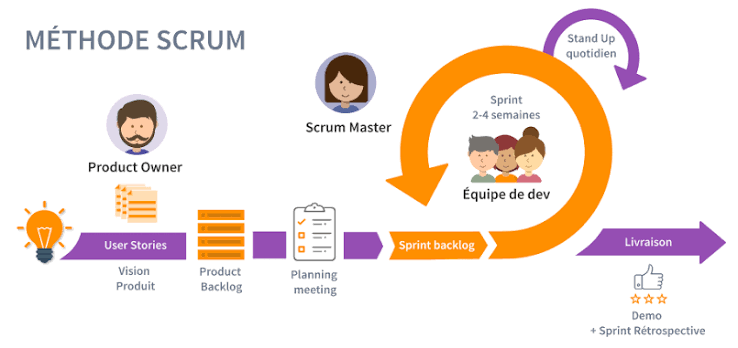
\includegraphics[width=0.9\textwidth]{images/scrum_cycle.png}
  \caption{Cycle de vie de la m\'ethodologie Scrum}
  \label{fig:scrum_cycle}
\end{figure}

\subsection{Planification et Chronogramme (Sprints)}

Le cycle de développement a été découpé en plusieurs sprints stratégiques afin de garantir des livraisons progressives et fonctionnelles :

\begin{itemize}
  \item \textbf{Sprint 0 : Initiation et conception.} Définition de l'architecture logicielle, analyse des besoins, élaboration des diagrammes UML et choix des technologies (Angular, Node.js).
  \item \textbf{Sprint 1 : Socle fonctionnel et Backend.} Mise en place de l'authentification (JWT, OAuth2), conception de la base de données MongoDB, et développement des opérations CRUD pour les projets et les tâches.
  \item \textbf{Sprint 2 : Frontend et Expérience utilisateur.} Développement des interfaces avec Angular (Dashboards, vues Kanban, gestion des utilisateurs) et liaison avec l'API Backend.
  \item \textbf{Sprint 3 : Intelligence Artificielle.} Intégration des modèles LLM, développement du chatbot contextuel et implémentation de la génération automatique des rapports.
  \item \textbf{Sprint 4 : Déploiement DevOps et Observabilité.} Containerisation avec Docker, écriture des manifestes Kubernetes, configuration du monitoring (Prometheus \& Grafana) et tests finaux.
\end{itemize}

\subsection{Méthodologie de conception (UML)}

Pour la conception logicielle de SmartPM, nous avons adopté le langage \textbf{UML} (Unified Modeling Language). 
Les diagrammes qui guideront notre conception dans les chapitres suivants sont :

\begin{itemize}
  \item \textbf{Diagramme de cas d'utilisation :} Modélise les interactions entre les utilisateurs (Admin, Manager, Member) et le système.
  \item \textbf{Diagramme de classes :} Représente l'architecture statique de la base de données et des entités métiers.
  \item \textbf{Diagramme de séquence :} Détaille les flux d'informations temporels (ex: processus d'authentification ou interaction avec l'IA).
  \item \textbf{Diagramme d'activités :} Illustre la logique des processus complexes (ex: le pipeline de génération de rapport par l'IA).
\end{itemize}

% ─────────────────────────────────────────────────────────
\section*{Conclusion}
% ─────────────────────────────────────────────────────────

Ce chapitre a permis de situer SmartPM dans son contexte général en présentant l'organisme
d'accueil Capgemini Tunisie, tout en mettant en évidence l'évolution du marché vers une gestion 
de projet plus intelligente et automatisée. L'étude critique de l'existant a confirmé la nécessité 
d'une solution innovante alliant l'Intelligence Artificielle générative et une architecture Cloud-Native robuste.
L'analyse de faisabilité et la gestion des risques nous ont permis de valider la viabilité technique du projet. 
Enfin, nous avons défini le cadre méthodologique Scrum et planifié les sprints qui structureront la réalisation.

\vspace{0.3cm}

Le chapitre suivant sera consacré à l'analyse approfondie des besoins fonctionnels et non-fonctionnels, 
ainsi qu'à la conception architecturale détaillée du système SmartPM via les diagrammes UML.
